\chapter{研究结果}

\section{阶段特征总结}

示例案例呈现出四个相对清晰的阶段。出道期依赖单一平台积累识别度；扩张期通过影视与综艺拓展角色边界；危机期的核心问题不是曝光下降，而是解释权丧失；重启期则依赖平台自主性与内容连续性重新组织公众认知。

\section{形象韧性路径}

\begin{figure}[H]
  \centering
  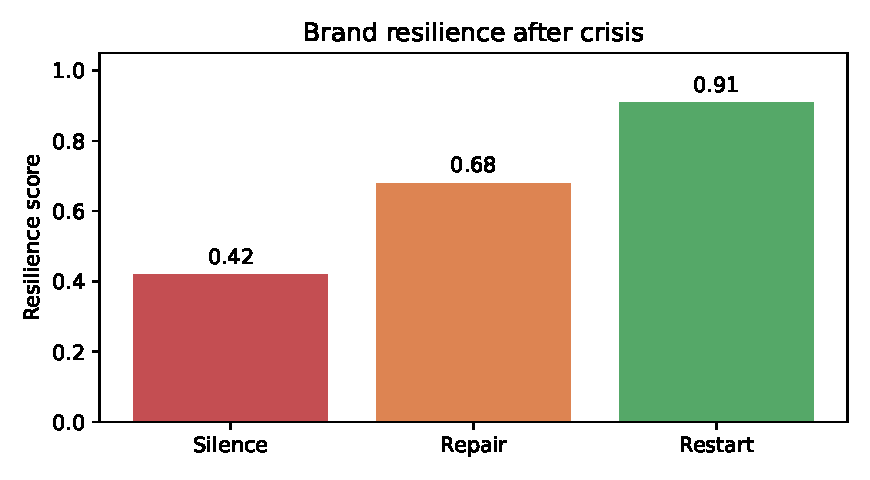
\includegraphics[width=0.70\textwidth]{assets/demo/resilience-curve.pdf}
  \caption{危机后的品牌韧性恢复路径}
  \label{fig:smu-resilience}
\end{figure}

从 \figref{fig:smu-resilience} 可见，品牌韧性并不是在危机结束后瞬间恢复，而是经历了沉默、修复与重启三个阶段。沉默期的核心目标是降低负面扩散速度；修复期依赖有限而稳定的外部露出；重启期则通过自有渠道建立新的内容节奏。

\section{平台迁移的收益与代价}

平台迁移带来至少两类收益：一是可触达受众的增加，二是叙事控制权的提升。但它也伴随更高的持续更新压力与更强的实时反馈。换言之，视频平台让艺人获得了更高的自主性，却也要求其在“持续产出”与“形象一致性”之间找到新的平衡。

\section{结果小结}

公开案例显示，成功的职业转型并不依赖某一次“爆款事件”，而取决于三种能力的组合：保持跨平台可见度、在危机中重建可控叙事，以及在新平台上形成稳定的表达节奏\cite{boyd2010,Bourdieu1986}。
